
\documentclass[11pt]{article}

\usepackage{common}
\usepackage{amsmath}
\usepackage{amssymb}

\title{HW1: Classification}
\author{Emily Tseng \\ et397@cornell.edu}
\begin{document}

\maketitle{}
\section{Introduction}

Given a sentence from a movie review, e.g. ``\textit{Never inspires more than an interested detachment.}'', how might we classify its sentiment, in this case \textit{negative}? 

In this assignment, we use the implementation of a handful of basic statistical models for this task to familiarize ourselves with core concepts and technologies in modern NLP. Specifically, we explored the use of the following models:

\begin{itemize}
  \item \textbf{Multinomial Naive Bayes (MNB)}, as outlined in \cite{wang2012baselines}
  \item \textbf{Logistic Regression (LR)}
  \item \textbf{Continuous Bag of Words (CBOW)}, as outlined in \cite{mikolov2013efficient}
  \item \textbf{Convolutional Neural Network (CNN)}, as outlined in \cite{kim2014convolutional}
  \item \textbf{CNN*}, a variant of the CNN using pretrained word embeddings
\end{itemize}

As a dataset, we used the Stanford Sentiment Treebank (SST-2) \citep{socher2013recursive}, which provides a corpus of sentences from movie reviews labeled as \textit{positive}, \textit{negative}, or \textit{neutral}. For this assignment, we removed neutral samples and formulated the task as a binary classification problem between positive and negative sentiment.


\section{Problem Description}

Given a sentence represented as a feature vector $\boldx$, we can find its predicted class $y \in \{-1, 1\}$, where -1 indicates negative sentiment and 1 indicates positive sentiment, via:
\begin{align}
  y = \sigma(\boldW\boldx + \boldb)
\end{align}

Where $\sigma$ is an activation function, $\boldW$ is a matrix of weights, and $\boldb$ is a vector of biases. $\boldx$ itself is generated using a feature function $\phi$, which can take a number of forms. We elaborate on the specific structures used per model in the subsequent section.

\section{Model and Algorithms}

\subsection{Multinomial Naive Bayes (MNB) over unigrams}

As formulated in \cite{wang2012baselines}, we consider the linear model where a prediction for test case $k$ is expressed as:
\begin{align}
  y^{(k)} = sign(\boldW^{T}\boldx^{(k)} + b)
\end{align}

We consider as features the unigrams within vocabulary $\mcV$, and define $\boldf^{(i)} \in \mathbb{R}^{|\mcV|}$ as the feature count vector for training case $i$ with label $y^{(i)} \in \{-1, 1\}$. $\boldf^{(i)}_j$ is thus the number of occurrences of feature $j$ in training sample $i$. We additionally consider the log-count ratio $r$ of the two count vectors $\boldp$ and $\boldq$, given smoothing parameter $\alpha$:
\begin{align}
  \boldp &= \alpha + \sum_{i:y^{(i)}=1}{\boldf^{(i)}} \\
  \boldq &= \alpha + \sum_{i:y^{(i)}=-1}{\boldf^{(i)}} \\
  \boldr &= log(\frac{\boldp / ||\boldp||_1}{\boldq / ||\boldq||_1})
\end{align}

In this implementation, we consider \textit{binarized count vectors}, in which $\hat{\boldf}_j$ is 1 if feature $j$ occurs at least once in the sentence, and 0 otherwise. For Naive Bayes we additionally consider our weight matrix as the vector of log-count ratios, and use as a bias the log-ratio of the number of positive to negative samples. Formally, we thus define as parameters the following, where $N+$ is the number of positive samples and $N-$ is the number of negative samples:

\begin{align}
  \boldx^{(k)} &= \hat{\boldf}^{(k)}, \hat{\boldf}^{(k)} = \textbf{1}\{f^{(k)} > 0\} \\
  \boldW^T &= \hat{\boldr} = log(\frac{\hat{\boldp} / ||\hat{\boldp}||_1}{\hat{\boldq} / ||\hat{\boldq}||_1}) \\
  \hat{\boldp} &= \alpha + \sum_{i:y^{(i)}=1}{\hat{\boldf}^{(i)}} \\
  \hat{\boldq} &= \alpha + \sum_{i:y^{(i)}=-1}{\hat{\boldf}^{(i)}} \\
  b &= log(\frac{N+}{N-})
\end{align}

\subsection{Logistic Regression}

Recalling (1), we express this model as a single-layer, fully-connected neural network using a sigmoid activation $\sigma$ to learn weight matrix $\boldW$ and bias vector $\boldb$. Here, $\boldx^{(i)}$ represents an input sentence as binarized counts of words in vocabulary $\mcV$, as in (6). The outputs $\boldy$ are thus 1x2 vectors representing the distribution over the two classes, and we take the argmax of $\boldy$ as the prediction. Our implementation randomly initializes all model parameters, uses Pytorch's built-in CrossEntropy loss function and standard stochastic gradient descent (SGD) optimizer, and backpropagates loss at each batch.

\subsection{CBOW}

The Continuous Bag of Words (CBOW) model as described in \citep{mikolov2013efficient} represents an input sentence $\boldx^{(i)}$ of length $n$ as a $k$-dimensional embedding vector $\bolde$ produced by averaging the individual $k$-dimensional embeddings for each word in the sentence. Formally:
\begin{align}
  \bolde = \frac{1}{n} \sum_{i=1}^{n} \bolde_i
\end{align}

This embedding is the input to a single-layer, fully-connected neural network using a softmax activation to learn a weight matrix and bias vector, as before. We take the argmax of the output of this linear layer as the prediction. As before, our implementation randomly initializes all model parameters, including the embeddings $\mcE$. Our training uses Pytorch's built-in CrossEntropy loss function and standard stochastic gradient descent (SGD) optimizer, and backpropagates loss at each batch.


\subsection{CNN}

The Convolutional Neural Network (CNN) approach to sentence classification as described in \cite{kim2014convolutional} represents input sentences as the concatenation of fixed-length embeddings. In other words, for an input sentence of length $n$:
\begin{align}
  \boldx_{1:n} = x_1 \oplus x_2 \oplus ... \oplus x_{n-1} \oplus x_n
\end{align}

This input is put through a convolutional layer consisting of a set of \textit{filters}. A filter generates a new feature thus:
\begin{align}
  c_i = f(\boldw\boldx_{i:i+h-1} + b)
\end{align}

where $f$ is a non-linear activation function such as the rectified linear unit (ReLU), $\boldw$ is the filter, $h$ is the window size for that convolutional layer, and $b$ is a bias term. Filters are applied over every possible \textit{window} (or \textit{kernel}) of the input to generate a feature map:
\begin{align}
  \boldc = [c_1, c_2, ... c_{n-h+1}]
\end{align}

A max-pooling over time operation is then applied over the feature map, which outputs the $c_i$ with the highest value as the value for that feature.

In our implementation, we follow \cite{kim2014convolutional} and use the ReLU nonlinearity, filters with window sizes 3, 4 and 5, a dropout rate of $p=0.5$ to regularize against overfitting during training, and a softmax activation function over the final output. The argmax of the output of this final layer is our prediction. As before, our implementation uses Pytorch's built-in CrossEntropy loss, but following \cite{kim2014convolutional} we use the Adadelta optimizer. Of note, in our implementation we padded inputs to a minimum length of 5 to ensure the provided window sizes would work.

\subsection{CNN*}

The CNN model above is initialized with random values as the initial word embeddings. We also experimented with a variant that initialized with pretrained word embeddings, but otherwise used the same structure and training as the CNN described above. 

\section{Experiments}

As depicted in Table \ref{tab:results}, our results show that when the learned models (LR, CBOW, CNN and CNN*) are trained for 20 epochs with a learning rate of $5e^{-2}$, MNB performs best, with a test-set accuracy of 0.82.

\begin{table}[h]
  \centering
  \begin{tabular}{llr}
   \toprule
   Model &  & Test Acc. \\
   \midrule
   \textsc{MNB} & & 0.82\\
   \textsc{LR} & & 0.71\\
   \textsc{CBOW} & & 0.66 \\
   \textsc{CNN} & & 0.70 \\
   \textsc{CNN*} & & 0.78 \\
   \bottomrule
  \end{tabular}
  \caption{\label{tab:results} Results from each model. LR, CBOW, CNN and CNN* models run with $lr=5e^{-2}$, $epochs=20$.}
  \end{table}

Examination of the losses per epoch shows the learned models are in fact learning, e.g. the losses per epoch decrease over training time (Figure \ref{fig:losses}). From this we infer the low accuracies for the learned models are due to the training parameters used, and do not accurately speak to their performance relative to MNB.

\begin{figure}[h]
  \centering
  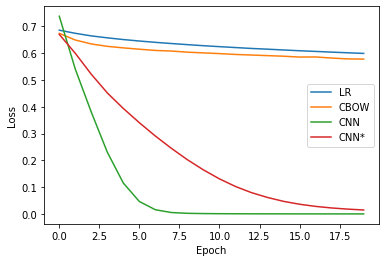
\includegraphics[width=4in]{losses.png}
  \caption{\label{fig:losses} Losses over time for the four learned models. All models trained with $lr=5e^{-2}$, $epochs=10$.}
\end{figure}

Still, we can draw conclusions from the relative differences in performance between the learned models: for instance, CNN* significantly outperforms CNN, as expected, and both outperform LR and CBOW.

\section{Conclusion}

This assignment investigated the use of 5 simple models for text classification. We implemented one count-based model, the Multinomial Naive Bayes (MNB), and four learned models, Logistic Regression (LR), Continuous Bag-of-Words (CBOW), Convolutional Neural Network (CNN) and a variant of the CNN initialized with pretrained word embeddings (CNN*). As shown in Table \ref{tab:results}, MNB performed best in our set of experiments, with a test-set accuracy of 0.82. Trained for 10 epochs with a learning rate of $5e^{-2}$, the four learned models (LR, CBOW, CNN, CNN*) did not perform as well as the MNB standard, but the relative accuracies achieved by these models highlight the differences between them: specifically, CNN* outperformed CNN as expected.

Further work might investigate additional hyperparameter tuning schemes to refine the learned models, for example by using learning rate annealing techniques, or simply training for more epochs. Further work should also pursue the use of novel representations of words and sentences as inputs to these models, for instance larger pretrained word embeddings derived from different sources (e.g. BERT), the use of parse trees and other semantic information, or even simply using n-grams more complex than unigrams in a count-based approach.


\bibliographystyle{apalike}
\bibliography{writeup}

\end{document}
